\documentclass{article}
\usepackage[utf8]{inputenc}
\usepackage[margin=1in, paperwidth=8.5in, paperheight=11in]{geometry}
\setlength{\parindent}{0pt}
\usepackage{graphicx}
\usepackage{caption}

\title{CompArch Midterm}
\author{Sarah Walters}
\date{14 November 2015}

\begin{document}

\maketitle

\section{Specification Document}
The system in question is the LED controller in a bike light.\\

The system's input is a single button, and its output is a single LED.\\

The LED controller has four operational modes, enumerated and explained below. Pushing the button causes a change in state (see Figure \ref{fig:fsm}).
\begin{enumerate}
\item Off: the LED is consistently off.
\item On: the LED is consistently on.
\item Dim: the LED pulses at 128Hz with a pulse width of 50\% to simulate 50\% brightness. Most humans don't detect flicker above 75Hz, so the LED doesn't look like it's blinking in the Dim state. \footnote{$\;$https://en.wikipedia.org/wiki/Flicker\_fusion\_threshold}
\item Blink: the LED pulses at 1Hz with a pulse width of 50\%. At 1Hz, the LED completes one on/off cycle per second.
\end{enumerate}

\begin{figure}[!ht]
\centering
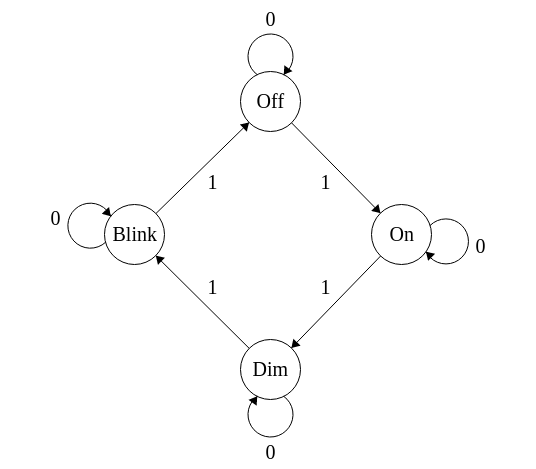
\includegraphics[width=0.5\textwidth]{img/fsm}
\caption{Finite state machine representation of the LED controller's operational modes. The arrows coming out of each state represent the position of the button -- when the button is pressed down (1), the finite state machine transitions to the next state in the cycle. When it is not pressed down (0), the finite state machine stays in its current state.}
\label{fig:fsm}
\end{figure}

\section{Block Diagram}
\begin{figure}[!ht]
\centering
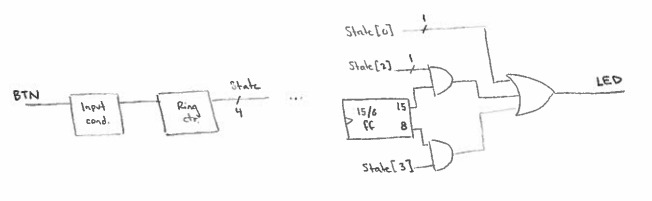
\includegraphics[width=\textwidth]{img/led-controller}
\caption{Caption}
\label{fig:led-controller}
\end{figure}

\begin{center}
\begin{tabular}{ ccc|c }
 \textbf{Subcomponent} & \textbf{Gate Inputs Per} & \textbf{Count} & \textbf{Total Gate Inputs} \\
 \hline
 Input conditioner & 117 & 1 & 117 \\
 4-bit ring counter & 83 & 1 & 83 \\
 8- and 15- T flip flop & 210 & 1 & 210 \\
 2-input AND & 3 & 2 & 6 \\
 3-input OR & 4 & 1 & 4 \\
 \hline
 &&& 420\\
\end{tabular}
\end{center}

\newpage

\section{Components}

\subsection{Input Conditioner}
The input conditioner filters a noisy input signal by ensuring that it is consistent for some amount of time before passing it through. We assume the noisy input signal is consistent within 1 millisecond; the system clock runs at $2^{15} = 32768$Hz, so the signal is consistent after $2^5$ clock cycles: $\frac{1}{2^{10}} = 0.0098$.\\

The input conditioner's inputs are a 1-bit noisy signal and the clock, and its output is a 1-bit conditioned signal.\\

\begin{figure}[!ht]
\centering
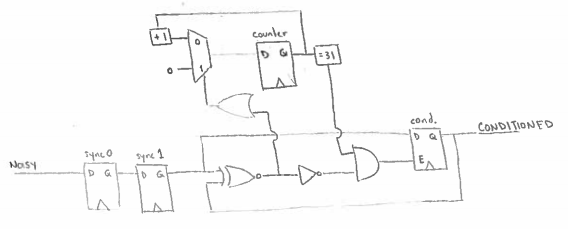
\includegraphics[width=\textwidth]{img/ic}
\label{fig:ic}
\end{figure}

\begin{center}
\begin{tabular}{ ccc|c }
 \textbf{Subcomponent} & \textbf{Gate Inputs Per} & \textbf{Count} & \textbf{Total Gate Inputs} \\
 \hline
 Posedge-triggered D flip-flop & 13 & 3 & 39 \\
 Posedge-triggered enabled DFF & 20 & 1 & 20 \\
 2-to-1 multiplexer & 7 & 1 & 7 \\
 2-input XNOR & 8 & 1 & 8 \\
 Inverter & 1 & 1 & 1 \\
 2-input AND & 3 & 1 & 3 \\
 2-input OR & 3 & 1 & 3 \\
 5-bit equal-to-31 checker & 6 & 1 & 6 \\
 5-bit carryin adder & 30 & 1 & 30 \\
 \hline
 &&& 117\\
\end{tabular}
\end{center}

\newpage

\subsection{1-bit carryin adder}
The 1-bit carryin adder is the building block for the 5-bit carryin adder. It adds its two inputs, a 1-bit number and a carryin; it outputs the LSB of the two-bit result as the sum and the MSB of the result as the carryout. \\

\begin{figure}[!ht]
\centering
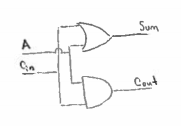
\includegraphics[width=0.3\textwidth]{img/1b-cin-add}
\label{fig:1b-cin-add}
\end{figure}

\begin{center}
\begin{tabular}{ ccc|c }
 \textbf{Subcomponent} & \textbf{Gate Inputs Per} & \textbf{Count} & \textbf{Total Gate Inputs} \\
 \hline
 2-input OR & 3 & 1 & 3 \\
 2-input AND & 3 & 1 & 3 \\
 \hline
 &&& 6\\
\end{tabular}
\end{center}

\subsection{5-bit carryin adder}
The 5-bit carryin adder adds 1 to a 5-bit number via the carryin to the 1-bit adder associated with the LSB. It requires less logic to add 1 using a carryin than it does to add 00001 using a full two-operand adder. \\

The 5-bit carryin adder's input is a 5-bit number, and its output is also a 5-bit number: the input plus one.\\

This adder doesn't flag for overflow.\\

\begin{figure}[!ht]
\centering
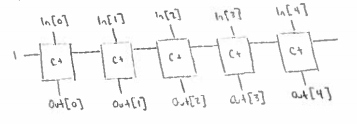
\includegraphics[width=0.7\textwidth]{img/5b-add1}
\label{fig:5b-add1}
\end{figure}

\begin{center}
\begin{tabular}{ ccc|c }
 \textbf{Subcomponent} & \textbf{Gate Inputs Per} & \textbf{Count} & \textbf{Total Gate Inputs} \\
 \hline
 1-bit carryin adder & 6 & 5 & 30\\
 \hline
 &&& 30\\
\end{tabular}
\end{center}

\newpage

\subsection{5-bit equal-to-31 checker}
This component checks whether its 5-bit input is equal to d31. Its output is a flag: 1 if the input is equal to 31, 0 if not. \\

\begin{figure}[!ht]
\centering
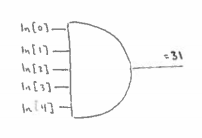
\includegraphics[width=0.4\textwidth]{img/eq31}
\caption{Caption}
\label{fig:eq31}
\end{figure}

\begin{center}
\begin{tabular}{ ccc|c }
 \textbf{Subcomponent} & \textbf{Gate Inputs Per} & \textbf{Count} & \textbf{Total Gate Inputs} \\
 \hline
 5-input AND & 6 & 1 & 6 \\
 \hline
 &&& 6\\
\end{tabular}
\end{center}

\subsection{T flip flop}
The T flip flop's input is a clock CLK; its output is a square wave Q with half the frequency of CLK. \\

\begin{figure}[!ht]
\centering
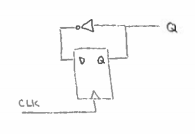
\includegraphics[width=0.4\textwidth]{img/tff}
\caption{Caption}
\label{fig:tff}
\end{figure}

\begin{center}
\begin{tabular}{ ccc|c }
 \textbf{Subcomponent} & \textbf{Gate Inputs Per} & \textbf{Count} & \textbf{Total Gate Inputs} \\
 \hline
 Posedge-triggered D flip flop & 13 & 1 & 13 \\
 Inverter & 1 & 1 & 1 \\
 \hline
 &&& 14\\
\end{tabular}
\end{center}

\newpage

\subsection{8- and 15- T flip flop}
The 8- and 15- T flip flop produces two square waves with lower frequency than the clock. Its input is a clock; let the frequency of the clock be $2^F$. It has two outputs: a square wave with a frequency of $2^{F-8}$ and a square wave with a frequency of $2^{F-15}$. \\

\begin{figure}[!ht]
\centering
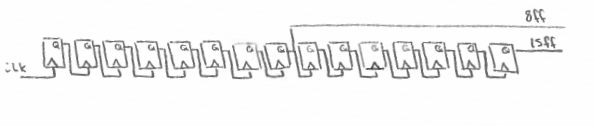
\includegraphics[width=\textwidth]{img/8-15-ff}
\caption{Caption}
\label{fig:8-15-ff}
\end{figure}

\begin{center}
\begin{tabular}{ ccc|c }
 \textbf{Subcomponent} & \textbf{Gate Inputs Per} & \textbf{Count} & \textbf{Total Gate Inputs} \\
 \hline
 T flip flop & 14 & 15 & 210 \\
 \hline
 &&& 210\\
\end{tabular}
\end{center}

\subsection{2-input XNOR\footnote{$\;$https://en.wikipedia.org/wiki/XNOR\_gate}}
The 2-input XNOR outputs 1 when its two 1-bit inputs are equal and 0 when they are not. \\

\begin{figure}[!ht]
\centering
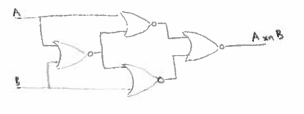
\includegraphics[width=0.5\textwidth]{img/xnor}
\caption{Caption}
\label{fig:xnor}
\end{figure}

\begin{center}
\begin{tabular}{ ccc|c }
 \textbf{Subcomponent} & \textbf{Gate Inputs Per} & \textbf{Count} & \textbf{Total Gate Inputs} \\
 \hline
 2-input NOR & 2 & 4 & 8 \\
 \hline
 &&& 8\\
\end{tabular}
\end{center}

\end{document}
